\chapter{हैमिल्टोनियन यांत्रिकी}\label{ch:b3:hamiltonian-mechanics}

किसी लोलक के हज़ार छायाचित्र लीजिए और हर चित्र के लिए उसका कोण उसके
कोणीय संवेग के सामने आलेखित कीजिए: बिंदु एक बंद वक्र पर बैठ जाते हैं,
और लोलक की हर संभव गति ऐसा ही एक वक्र है --- छोटे झूले नत्थी अंडाकारों
पर, पूरे चक्कर ऊपर-नीचे की लहरदार रेखाओं पर, और उनके बीच एक अकेला
आड़ा-तिरछा वक्र, जो दोनों परिसरों को अलग करता है। यही चित्र, अर्थात्
\emph{\omterm{def:b3:hamiltonian-mechanics:portrait}{कला चित्र}}, उस पुनर्रचना का हृदय है जो
हैमिल्टन ने 1833 में यांत्रिकी को दी: किसी तंत्र की अवस्था निर्देशांकों
\emph{और} संवेगों की समष्टि का एक बिंदु है, उसका विकास उस समष्टि में एक
प्रवाह है, और वह प्रवाह एक ही फलन से, अर्थात् ऊर्जा से, दो सुंदर सममित
प्रथम-कोटि समीकरणों के द्वारा उत्पन्न होता है। इसका पुरस्कार आसान गणना
नहीं --- वहाँ प्रायः लाग्रांज ही जीतता है --- बल्कि सही
\emph{ज्यामिति} है: प्रवाह कला-समष्टि का आयतन संरक्षित रखता है, जिस पर
आगे सांख्यिकीय भौतिकी खड़ी होगी; और उसका बीजगणितीय
ढाँचा, \omterm{def:b3:hamiltonian-mechanics:poisson}{प्वासों कोष्ठक}, ठीक वही है जिसे क्वांटम यांत्रिकी
क्रमविनिमेयक तक उठा देगी। यह अध्याय वस्तुओं की यांत्रिकी और बीसवीं सदी
की भौतिकी के बीच का कब्ज़ा है।

\section{लाग्रांज से हैमिल्टन तक}

\begin{definition}[हैमिल्टोनियन और विहित समीकरण]\label{def:b3:hamiltonian-mechanics:hamiltonian}
\index{हैमिल्टोनियन}\index{विहित समीकरण}\index{कला समष्टि}
\omterm{def:b3:lagrangian-mechanics:action}{लाग्रांजियन} $L(q, \dot q, t)$ वाले किसी तंत्र के लिए वेगों को
संवेगों $p_i = \partial L/\partial\dot q_i$ के पदों में व्यक्त कीजिए और
\emph{हैमिल्टोनियन} को लजांद्र रूपांतर के रूप में इस तरह परिभाषित कीजिए
\[
H(q, p, t) = \sum_i p_i\dot q_i - L ,
\]
यह निर्देशांकों और \emph{संवेगों} का फलन है।
$2n$-विमीय समष्टि, अर्थात् $(q_1, \dots, q_n, p_1, \dots, p_n)$ की समष्टि,
ही \emph{कला समष्टि} है; उसका एक बिंदु --- अर्थात् एक \emph{अवस्था} ---
तंत्र का पूरा भविष्य और पूरा भूत
\cref{thm:b3:hamiltonian-mechanics:canonical} के \emph{विहित समीकरणों}
के द्वारा नियत कर देता है।
\end{definition}

\begin{theorem}[हैमिल्टन के समीकरण]\label{thm:b3:hamiltonian-mechanics:canonical}
\omterm{thm:b3:lagrangian-mechanics:euler-lagrange}{ऑयलर--लाग्रांज समीकरण} इन $2n$ प्रथम-कोटि
समीकरणों के तुल्य हैं
\[
\dot q_i = \frac{\partial H}{\partial p_i} , \qquad
\dot p_i = -\frac{\partial H}{\partial q_i} .
\]
\end{theorem}

\begin{proof}
$H = \sum p_i\dot q_i - L$ का $(q, p, t)$ के फलन के रूप में अवकलन कीजिए:
$\dd H = \sum(\dot q_i\,\dd p_i + p_i\,\dd\dot q_i) - \sum(
\partial_{q_i}L\,\dd q_i + \partial_{\dot q_i}L\,\dd\dot q_i) -
\partial_tL\,\dd t$। $\dd\dot q_i$ वाले पद
$p_i$ की परिभाषा से कट जाते हैं --- लजांद्र रूपांतर का सारा मर्म यही
है --- और बचता है
$\dd H = \sum(\dot q_i\,\dd p_i - \partial_{q_i}L\,\dd q_i) -
\partial_tL\,\dd t$। आंशिक अवकलज पढ़ लेने पर:
$\partial H/\partial p_i = \dot q_i$ और $\partial H/\partial q_i =
-\partial L/\partial q_i$, जो ऑयलर--लाग्रांज से $-\dot p_i$ है।
(साथ ही $\partial_tH = -\partial_tL$।)
\end{proof}

\begin{proposition}[$H$ है क्या]\label{prop:b3:hamiltonian-mechanics:energy}
$H$ पिछले अध्याय के \omterm{prop:b3:lagrangian-mechanics:energy}{ऊर्जा फलन} $h$ से मेल खाता है:
किसी गति के अनुदिश $\dd H/\dd t = \partial H/\partial t$, अतः जब भी
$H$ में स्पष्ट काल-निर्भरता न हो, वह संरक्षित रहता है; और जब गतिज ऊर्जा
वेगों में द्विघात हो तथा \omterm{def:b3:lagrangian-mechanics:coordinates}{प्रतिबंध} समय-निरपेक्ष हों, तब
$H = E_k + E_p$, अर्थात् यांत्रिक ऊर्जा --- अब चरों $(q, p)$ में लिखी
हुई।
\end{proposition}

\begin{proof}
$\dd H/\dd t = \sum(\partial_{q_i}H\,\dot q_i + \partial_{p_i}H\,\dot
p_i) + \partial_tH = \sum(\partial_{q_i}H\,\partial_{p_i}H -
\partial_{p_i}H\,\partial_{q_i}H) + \partial_tH = \partial_tH$:
विहित समीकरणों की सममिति योग को सर्वसमतः शून्य कर देती है।
$E_k + E_p$ के साथ तादात्म्य
\cref{prop:b3:lagrangian-mechanics:energy} है।
\end{proof}

\begin{example}[दो हैमिल्टोनियन]\label{ex:b3:hamiltonian-mechanics:examples}
स्प्रिंग पर द्रव्यमान: $p = m\dot x$, अतः
\[
H = \frac{p^2}{2m} + \frac12 kx^2 ;
\]
\omterm{def:b3:hamiltonian-mechanics:hamiltonian}{विहित समीकरण} $\dot x = p/m$, $\dot p = -kx$ वही परिचित
युग्म हैं। लोलक: $p = m\ell^2\dot\theta$ और
\[
H = \frac{p^2}{2m\ell^2} - mg\ell\cos\theta .
\]
दोनों स्थितियों में $H$ ऊर्जा है, हर गति पर अचर: गतियाँ $H$ के वे
तलवक्र ही \emph{हैं} जो $(q,p)$ तल में हैं।
\end{example}

\begin{method}[हैमिल्टोनियन विधि]\label{met:b3:hamiltonian-mechanics:recipe}
(1) $L$ से संवेग $p_i = \partial L/\partial\dot q_i$ निकालिए
और $\dot q_i$ के लिए उलटिए। (2) $H = \sum p_i\dot q_i - L$, जो केवल
$(q, p)$ में व्यक्त हो --- किसी स्वाभाविक तंत्र के लिए वह बस $E_k + E_p$
है, जिसमें $E_k$ संवेगों में लिखा गया हो। (3) \omterm{def:b3:hamiltonian-mechanics:hamiltonian}{विहित
समीकरण} लिखिए। (4) $H$ के तलवक्र खींचिए: एक \omterm{def:b3:lagrangian-mechanics:coordinates}{स्वातंत्र्य कोटि} के लिए वही
प्रक्षेप-पथ हैं, और पूरी गुणात्मक गति --- दोलन, घूर्णन, साम्यावस्थाएँ,
\omterm{def:b3:hamiltonian-mechanics:portrait}{पृथक्कारी वक्र} --- बिना कुछ हल किए ही पढ़ी जा सकती है।
\end{method}

\section{कला समष्टि}

\begin{definition}[कला चित्र, स्थिर बिंदु, पृथक्कारी वक्र]\label{def:b3:hamiltonian-mechanics:portrait}
\index{कला चित्र}\index{स्थिर बिंदु}\index{पृथक्कारी वक्र}
किसी तंत्र का \emph{कला चित्र} \omterm{def:b3:hamiltonian-mechanics:hamiltonian}{कला समष्टि} में उसके
प्रक्षेप-पथों का कुल है। \emph{स्थिर बिंदु} वह अवस्था है जहाँ
दोनों \omterm{def:b3:hamiltonian-mechanics:hamiltonian}{विहित समीकरण} लुप्त हो जाते हैं --- अर्थात् साम्यावस्था: विभव का
निम्निष्ठ एक \emph{केंद्र} की तरह दिखता है, जिसके चारों ओर बंद वक्र
होते हैं, और उच्चिष्ठ एक \emph{काठी बिंदु} की तरह, जिससे होकर एक
\emph{पृथक्कारी वक्र} गुज़रता है --- वह प्रक्षेप-पथ जो \omterm{def:b3:hamiltonian-mechanics:hamiltonian}{कला समष्टि} को
गुणात्मक रूप से भिन्न गति के क्षेत्रों में बाँट देता है।
\end{definition}

\begin{example}[लोलक का कला चित्र]\label{ex:b3:hamiltonian-mechanics:pendulum-portrait}
$H = p^2/2m\ell^2 - mg\ell\cos\theta$ के लिए: $(0, 0)$ के चारों ओर बंद
अंडाकार --- \emph{आंदोलन}, अर्थात् साधारण झूले; बड़े
$|p|$ पर लहरदार वक्र --- \emph{घूर्णन}, जब लोलक शीर्ष के ऊपर से घूम
जाता है; और $\theta = \pm\pi$ के काठी बिंदुओं से होकर \omterm{def:b3:hamiltonian-mechanics:portrait}{पृथक्कारी वक्र},
जिसकी ऊर्जा $E = +mg\ell$ है और जिस पर लोलक को शीर्ष तक पहुँचने में
अनंत समय लगता है। \omterm{def:b3:hamiltonian-mechanics:portrait}{पृथक्कारी वक्र} पर की अवस्था वह झूला है जिसे
\emph{ठीक} उतना ही ज़ोर दिया गया है कि वह उलटी स्थिति तक बिना कुछ बचाए
पहुँच जाए।
\end{example}

\begin{omfigure}
\begin{tikzpicture}
  \begin{axis}[omaxis, axis x line=bottom, axis y line=left,
    width=11.6cm, height=6.4cm, xmin=-180, xmax=180, ymin=-3.2, ymax=3.2,
    xlabel={$\theta$ (डिग्री)},
    xlabel style={at={(axis description cs:0.5,-0.08)}, anchor=north},
    ylabel={$p$ ($m\ell^2\omega_0$ के मात्रकों में)},
    xtick={-180,-90,0,90,180}, ytick={-2,0,2}, clip=false]
    % librations E/mgl = -0.5 and 0.4 : p = ±sqrt(2(E'+cos x)), E'=E/mgl
    \addplot[omDef, thick, domain=-60:60, samples=80] {sqrt(2*(-0.5+cos(x)))};
    \addplot[omDef, thick, domain=-60:60, samples=80] {-sqrt(2*(-0.5+cos(x)))};
    \addplot[omDef, thick, domain=-113.5:113.5, samples=100] {sqrt(2*(0.4+cos(x)))};
    \addplot[omDef, thick, domain=-113.5:113.5, samples=100] {-sqrt(2*(0.4+cos(x)))};
    % separatrix E'=1: p=±2cos(x/2)
    \addplot[omThm, very thick, domain=-180:180, samples=100] {2*cos(x/2)};
    \addplot[omThm, very thick, domain=-180:180, samples=100] {-2*cos(x/2)};
    % rotations E'=2 and 3.5
    \addplot[omExo, thick, domain=-180:180, samples=100] {sqrt(2*(2+cos(x)))};
    \addplot[omExo, thick, domain=-180:180, samples=100] {-sqrt(2*(2+cos(x)))};
    \addplot[omExo, thick, domain=-180:180, samples=100] {sqrt(2*(3.5+cos(x)))};
    \addplot[omExo, thick, domain=-180:180, samples=100] {-sqrt(2*(3.5+cos(x)))};
    % fixed points
    \fill (axis cs:0,0) circle (1.8pt);
    \fill (axis cs:180,0) circle (1.8pt);
    \fill (axis cs:-180,0) circle (1.8pt);
    % flow arrows
    \draw[->, thick] (axis cs:-6,1.66) -- (axis cs:6,1.66);
    \draw[->, thick] (axis cs:6,-1.66) -- (axis cs:-6,-1.66);
    \draw[->, thick] (axis cs:-6,2.45) -- (axis cs:6,2.45);
    \draw[->, thick] (axis cs:6,-2.45) -- (axis cs:-6,-2.45);
    \node[omDef, font=\scriptsize, anchor=west] at (axis cs:-52,0.5) {आंदोलन};
    \node[omThm, font=\scriptsize, anchor=west] at (axis cs:97,1.75) {पृथक्कारी वक्र};
    \node[omExo, font=\scriptsize, anchor=west] at (axis cs:-172,2.93) {घूर्णन};
  \end{axis}
\end{tikzpicture}

{\small लोलक का \omterm{def:b3:hamiltonian-mechanics:portrait}{कला चित्र}: $H$ के तलवक्र। बंद
अंडाकार (झूले) केंद्र के चारों ओर दक्षिणावर्त परिक्रमा करते हैं;
\omterm{def:b3:hamiltonian-mechanics:portrait}{पृथक्कारी वक्र} के ऊपर और नीचे लोलक घूमता है। $\pm 180^\circ$ पर के
काठी बिंदु उलटी साम्यावस्था हैं।}
\end{omfigure}

\begin{theorem}[ल्यूविल की प्रमेय]\label{thm:b3:hamiltonian-mechanics:liouville}
\index{ल्यूविल की प्रमेय}
\omterm{def:b3:hamiltonian-mechanics:hamiltonian}{हैमिल्टोनियन} प्रवाह कला-समष्टि का आयतन बनाए रखता है: यदि प्रारंभिक
अवस्थाओं का कोई क्षेत्र विहित समीकरणों के साथ बहा ले जाया जाए, तो उसका
आयतन (एक \omterm{def:b3:lagrangian-mechanics:coordinates}{स्वातंत्र्य कोटि} के लिए उसका क्षेत्रफल) कभी नहीं बदलता ---
उसका आकार चाहे जो बन जाए।
\end{theorem}

\begin{proof}
\omterm{def:b3:hamiltonian-mechanics:hamiltonian}{कला समष्टि} में प्रवाह का वेग-क्षेत्र $(\dot q_i, \dot p_i) =
(\partial_{p_i}H, -\partial_{q_i}H)$ है। उसका अपसरण है
\[
\sum_i\Big(\frac{\partial\dot q_i}{\partial q_i}
 + \frac{\partial\dot p_i}{\partial p_i}\Big)
 = \sum_i\Big(\frac{\partial^2H}{\partial q_i\partial p_i}
 - \frac{\partial^2H}{\partial p_i\partial q_i}\Big) = 0 :
\]
प्रवाह असंपीड्य है, और असंपीड्य प्रवाह आयतनों को अपरिवर्तित ले जाता है,
ठीक वैसे ही जैसे वर्ष 2 के खंड के तरलों में। (शून्य अपसरण से संरक्षित
आयतन तक का औपचारिक कदम वहीं सिद्ध की गई परिवहन प्रमेय है।)
\end{proof}

\begin{remark}[ल्यूविल क्यों महत्वपूर्ण है]\label{rem:b3:hamiltonian-mechanics:liouville-matters}
न्यूटन की रचना में कुछ भी यह संकेत नहीं देता कि कुछ असंपीड्य है।
\omterm{def:b3:hamiltonian-mechanics:hamiltonian}{हैमिल्टोनियन} चित्र में यह स्वतःसिद्ध है --- और यही सांख्यिकीय भौतिकी की
अनुज्ञप्ति है: जब हम
$10^{23}$ अणुओं की गैस का वर्णन \omterm{def:b3:hamiltonian-mechanics:hamiltonian}{कला समष्टि} में बिंदुओं के बादल से करते
हैं, तब \omterm{thm:b3:hamiltonian-mechanics:liouville}{ल्यूविल की प्रमेय} कहती है कि वह बादल किसी असंपीड्य तरल की तरह
बहता है, इसलिए ``किसी कला-समष्टि आयतन में अवस्थाओं की संख्या'' ऐसी राशि
है जिसे गतिकी स्वयं न बना सकती है न मिटा सकती है। इसी खंड में आगे आने
वाला सांख्यिकीय भौतिकी का सूक्ष्मविहित अभिगृहीत ठीक इसी पर टिका है।
\end{remark}

\begin{omfigure}
\begin{tikzpicture}[font=\small, >=Stealth]
  % free particle shear
  \begin{scope}
    \draw[->] (0,0) -- (5.2,0) node[right] {$q$};
    \draw[->] (0,0) -- (0,3.0) node[above] {$p$};
    \fill[omDef!30, draw=omDef, thick] (0.6,0.8) rectangle (1.6,2.2);
    \fill[omDef!30, draw=omDef, thick] (2.7,0.8) -- (3.7,0.8) -- (5.1,2.2) -- (4.1,2.2) -- cycle;
    \draw[->, thick] (1.85,1.5) -- (2.5,1.5);
    \node at (1.1,0.45) {$t = 0$};
    \node at (3.9,0.45) {$t > 0$};
  \end{scope}
  \node[font=\footnotesize] at (2.6,-0.7) {स्वतंत्र कण: $\dot q = p/m$ धब्बे को अपरूपित कर देता है};
  % harmonic oscillator rotation
  \begin{scope}[xshift=9.6cm]
    \draw[->] (-2.6,0) -- (2.8,0) node[right] {$q$};
    \draw[->] (0,-1.55) -- (0,2.9) node[above] {$p$};
    \draw[gray, dashed] (0,0) circle (1.75);
    \fill[omThm!30, draw=omThm, thick] (1.35,0.35) -- (2.15,0.35) -- (2.15,0.95) -- (1.35,0.95) -- cycle;
    \begin{scope}[rotate=100]
    \fill[omThm!30, draw=omThm, thick] (1.35,0.35) -- (2.15,0.35) -- (2.15,0.95) -- (1.35,0.95) -- cycle;
    \end{scope}
    \draw[->, thick] (2.0,1.35) arc (35:75:2.35);
    \node at (2.5,-0.45) {$t = 0$};
    \node at (-1.15,2.45) {$t > 0$};
  \end{scope}
  \node[font=\footnotesize] at (9.6,-0.7) {हरात्मक दोलक: धब्बा दृढ़ रूप से घूमता है};
\end{tikzpicture}

{\small \omterm{thm:b3:hamiltonian-mechanics:liouville}{ल्यूविल की प्रमेय}: प्रवाह प्रारंभिक अवस्थाओं के किसी क्षेत्र को
विरूपित करता है --- कभी अपरूपित करके, कभी घुमाकर --- पर उसका क्षेत्रफल
ठीक-ठीक संरक्षित रहता है।}
\end{omfigure}

\section{प्वासों कोष्ठक}

\begin{definition}[प्वासों कोष्ठक]\label{def:b3:hamiltonian-mechanics:poisson}
\index{प्वासों कोष्ठक}
\omterm{def:b3:hamiltonian-mechanics:hamiltonian}{कला समष्टि} पर के दो फलनों $f(q, p, t)$ और
$g(q, p, t)$ का \emph{प्वासों कोष्ठक} है
\[
\{f, g\} = \sum_i\Big(
 \frac{\partial f}{\partial q_i}\frac{\partial g}{\partial p_i}
 - \frac{\partial f}{\partial p_i}\frac{\partial g}{\partial q_i}\Big) .
\]
यह प्रतिसममित है, हर कोटि में रैखिक है, गुणनफल-नियम
$\{f, gh\} = \{f, g\}h + g\{f, h\}$ का पालन करता है, और स्वयं
निर्देशांकों के लिए \emph{विहित संबंध} संतुष्ट करता है
\[
\{q_i, p_j\} = \delta_{ij} , \qquad
\{q_i, q_j\} = \{p_i, p_j\} = 0 .
\]
\end{definition}

\begin{theorem}[विकास एक कोष्ठक के रूप में]\label{thm:b3:hamiltonian-mechanics:evolution}
किसी भी गति के अनुदिश,
\[
\frac{\dd f}{\dd t} = \{f, H\} + \frac{\partial f}{\partial t} .
\]
विशेष रूप से, स्पष्ट काल-निर्भरता रहित कोई राशि तभी और केवल तभी
संरक्षित है जब \omterm{def:b3:hamiltonian-mechanics:hamiltonian}{हैमिल्टोनियन} के साथ उसका कोष्ठक लुप्त हो; और
स्वयं \omterm{def:b3:hamiltonian-mechanics:hamiltonian}{विहित समीकरण} $\dot q_i = \{q_i, H\}$, $\dot p_i
= \{p_i, H\}$ हैं: \omterm{def:b3:hamiltonian-mechanics:hamiltonian}{हैमिल्टोनियन} काल-विकास को \emph{उत्पन्न} करता है।
\end{theorem}

\begin{proof}
शृंखला-नियम और \omterm{def:b3:hamiltonian-mechanics:hamiltonian}{विहित समीकरण} मिलकर इस तरह देते हैं: $\dd f/\dd t = \sum(
\partial_{q_i}f\,\dot q_i + \partial_{p_i}f\,\dot p_i) + \partial_tf =
\sum(\partial_{q_i}f\,\partial_{p_i}H - \partial_{p_i}f\,
\partial_{q_i}H) + \partial_tf$।
\end{proof}

\begin{example}[कोणीय संवेग के कोष्ठक]\label{ex:b3:hamiltonian-mechanics:brackets}
एक कण के लिए $L_z = xp_y - yp_x$ और उसके चक्रीय साथी। विहित संबंधों से
सीधी गणना देती है
\[
\{L_x, L_y\} = L_z , \qquad
\{L_y, L_z\} = L_x , \qquad
\{L_z, L_x\} = L_y ,
\]
और $\{L^2, L_z\} = 0$: कोणीय संवेग के घटक आपस में
``क्रमविनिमेय'' नहीं हैं, पर हर घटक कुल वर्ग के साथ क्रमविनिमेय है।
इन संबंधों का आकार याद रखिए --- ये अक्षरशः लौटेंगे, क्वांटम यांत्रिकी
में क्रमविनिमेयकों के रूप में, जहाँ ये परमाणु-संरचना के विषय में सब कुछ
तय करते हैं।
\end{example}

\begin{remark}[क्वांटम यांत्रिकी का द्वार]\label{rem:b3:hamiltonian-mechanics:doorway}
डिराक ने 1925 में देखा कि पूरी क्वांटम यांत्रिकी इस तरह मिल जाती है:
\omterm{def:b3:hamiltonian-mechanics:hamiltonian}{हैमिल्टोनियन} यांत्रिकी का बीजगणित रखिए और
\omterm{def:b3:hamiltonian-mechanics:poisson}{प्वासों कोष्ठक} के स्थान पर संकारकों का क्रमविनिमेयक, जिसे
$\iu\hbar$ से भाग दिया गया हो, रख दीजिए: $\{q, p\} = 1$, $[\hat x, \hat p] = \iu\hbar$ बन जाता है,
संरक्षण अब भी ``$H$ के साथ कोष्ठक लुप्त होना'' है, और काल-विकास
अब भी \omterm{def:b3:hamiltonian-mechanics:hamiltonian}{हैमिल्टोनियन} से उत्पन्न होता है। चिरसम्मत सिद्धांत
अपनी हड्डियों में क्वांटम सिद्धांत का ढाँचा लिए चलता है; क्वांटम
यांत्रिकी के अध्याय इस संगति को स्पष्ट कर देंगे।
\end{remark}

\section{क्रिया और रुद्धोष्म निश्चर}

\begin{definition}[क्रिया चर]\label{def:b3:hamiltonian-mechanics:action-variable}
\index{क्रिया चर}
किसी बंद कला-प्रक्षेप-पथ पर दोलन करते एक-स्वातंत्र्य-कोटि तंत्र के लिए
\emph{\omterm{def:b3:lagrangian-mechanics:action}{क्रिया} चर} वह घिरा हुआ क्षेत्रफल है जिसे
$2\pi$ से भाग दिया गया हो:
\[
I = \frac{1}{2\pi}\oint p\,\dd q .
\]
\end{definition}

\begin{proposition}[हरात्मक दोलक की क्रिया]\label{prop:b3:hamiltonian-mechanics:sho-action}
$H = p^2/2m + \tfrac12 m\omega^2q^2$ के लिए, ऊर्जा $E$ पर, प्रक्षेप-पथ
$\sqrt{2E/m\omega^2}$ और $\sqrt{2mE}$ अर्ध-अक्षों वाला दीर्घवृत्त है,
जो क्षेत्रफल $2\pi E/\omega$ घेरता है: अतः
\[
I = \frac{E}{\omega} , \qquad E = \omega I ,
\]
और दोलन-आवृत्ति $\partial E/\partial I = \omega$ है, जैसा उसे होना
चाहिए।
\end{proposition}

\begin{proof}
दीर्घवृत्त का क्षेत्रफल, $\pi ab = \pi\sqrt{2E/m\omega^2}\sqrt{2mE} =
2\pi E/\omega$।
\end{proof}

\begin{proposition}[रुद्धोष्म निश्चरता]\label{prop:b3:hamiltonian-mechanics:adiabatic}
\index{रुद्धोष्म निश्चर}
यदि तंत्र का कोई प्राचल (कोई लंबाई, कोई दृढ़ता, कोई क्षेत्र)
\emph{धीरे-धीरे} बदला जाए --- अनेक दोलन-आवर्तकालों में --- तो ऊर्जा
बदलती है, आवृत्ति बदलती है, पर \omterm{def:b3:lagrangian-mechanics:action}{क्रिया} $I$ बहुत अच्छे सन्निकटन में अचर
रहती है: $I$ एक \emph{\omterm{prop:b3:hamiltonian-mechanics:adiabatic}{रुद्धोष्म निश्चर}} है।
धीरे-धीरे बदले गए दोलक के लिए इस प्रकार $E/\omega$ संरक्षित रहता है:
स्प्रिंग को धीरे-धीरे कड़ा करके $\omega$ दुगुना कीजिए, ऊर्जा भी उसके
साथ दुगुनी हो जाती है।
\end{proposition}

\begin{proof}[आंशिक उपपत्ति]
धीरे-धीरे बदलते $\omega(t)$ वाले दोलक के लिए: एक आवर्तकाल में
बदलते प्राचल द्वारा किया गया कार्य औसत लेकर निकाला जा सकता है;
वह गणना (\cref{exo:b3:hamiltonian-mechanics:11} में निर्देशित)
अग्रणी कोटि पर $\dot E/E = \dot\omega/\omega$ देती है, अर्थात्
$\dd(E/\omega)/\dd t = 0$। किसी भी धीरे-धीरे विरूपित होते दोलनशील
तंत्र के लिए व्यापक कथन स्वीकृत है --- यही कारण है कि ग्रहों की कक्षाएँ
मंद विक्षोभों को झेल जाती हैं, और यही नीचे की ``पुरानी क्वांटम
सिद्धांत'' का आरंभ-बिंदु है।
\end{proof}

\begin{omfigure}
\begin{tikzpicture}[font=\small, >=Stealth]
  \begin{scope}
    \draw[->] (-2.9,0) -- (2.9,0) node[right] {$q$};
    \draw[->] (0,-1.9) -- (0,2.3) node[above] {$p$};
    \draw[omDef, thick] (0,0) ellipse (2.3 and 0.85);
    \draw[omThm, thick] (0,0) ellipse (1.63 and 1.2);
    \node[omDef, anchor=west] at (1.5,-1.1) {$\omega$};
    \node[omThm, anchor=west] at (0.2,1.45) {$2\omega$};
  \end{scope}
  \node[align=center] at (0,-2.75) {धीरे-धीरे कड़ा किया गया दोलक:\\दीर्घवृत्त पतला होता है, क्षेत्रफल बचा रहता है};
  \begin{scope}[xshift=8.2cm]
    \fill (0,2.1) circle (1.5pt);
    \draw[thick] (-1.1,2.1) -- (1.1,2.1);
    \foreach \i in {-0.95,-0.6,-0.25,0.1,0.45,0.8} \draw (\i,2.1) -- (\i+0.16,2.24);
    \draw[thick] (0,2.1) -- ++(-115:1.15) coordinate (bob1);
    \fill[omDef] (bob1) circle (2.6pt);
    \draw[dashed] (0,2.1) -- ++(-115:2.3) coordinate (bob2);
    \fill[omDef!45] (bob2) circle (2.6pt);
    \draw[->] (0.02,1.0) -- (0.02,1.6);
    \node[anchor=west] at (0.1,1.28) {खींचिए};
    \node[align=center] at (0,-0.85) {झूलते लोलक को धीरे-धीरे छोटा करना:\\$E/\omega$ अचर, आयाम बढ़ता है};
  \end{scope}
\end{tikzpicture}

{\small रुद्धोष्म निश्चरता। बाएँ: ज्यों-ज्यों $\omega$ धीरे-धीरे
दुगुना किया जाता है, कला-दीर्घवृत्त अचर क्षेत्रफल पर आकार बदलता है,
अतः $E = \omega I$ दुगुना हो जाता है। दाएँ: झूलते लोलक की डोरी खींचना
झूले में ठीक उसी अनुपात में ऊर्जा भरता है जो
$I = E/\omega$ को अचर रखे।}
\end{omfigure}

\begin{remark}[पुरानी क्वांटम सिद्धांत]\label{rem:b3:hamiltonian-mechanics:old-quantum}
परमाणुओं की ऊर्जाएँ विविक्त क्यों होती हैं? पहला मात्रात्मक उत्तर
(बोर 1913, ज़ोमरफ़ेल्ट 1915) इसी अध्याय की भाषा में लिखा गया था: सभी
चिरसम्मत गतियों में से प्रकृति उन्हीं को रखती है जिनका क्रिया-समाकल
प्लांक के नियतांक का पूर्ण गुणज हो,
\[
\oint p\,\dd q = nh .
\]
हरात्मक दोलक पर लगाने से यह $E_n = n\hbar\omega$ देता है
(केवल सच्चे $\big(n + \tfrac12\big)\hbar
\omega$ का आधा छूट जाता है); किसी संदूक में बंद कण पर लगाने से यह
वर्ष 2 के खंड के स्तर \emph{ठीक-ठीक} देता है; हाइड्रोजन परमाणु पर
(\cref{pb:b3:hamiltonian-mechanics:1}) यह मापे गए वर्णक्रम को चार अंकों
तक देता है। नियम मात्रात्मक रूप से सही था और वैचारिक रूप से
अस्थायी --- और चूँकि \omterm{def:b3:lagrangian-mechanics:action}{क्रिया} एक \omterm{prop:b3:hamiltonian-mechanics:adiabatic}{रुद्धोष्म निश्चर} है, इसलिए
क्वांटम संख्या $n$ मंद विक्षोभों के अंतर्गत नहीं बदलती, और इसी से ऐसा
नियम काम कर सका। सच्चा सिद्धांत यहाँ से पाँच अध्याय आगे शुरू होता है।
\end{remark}

\begin{omfigure}
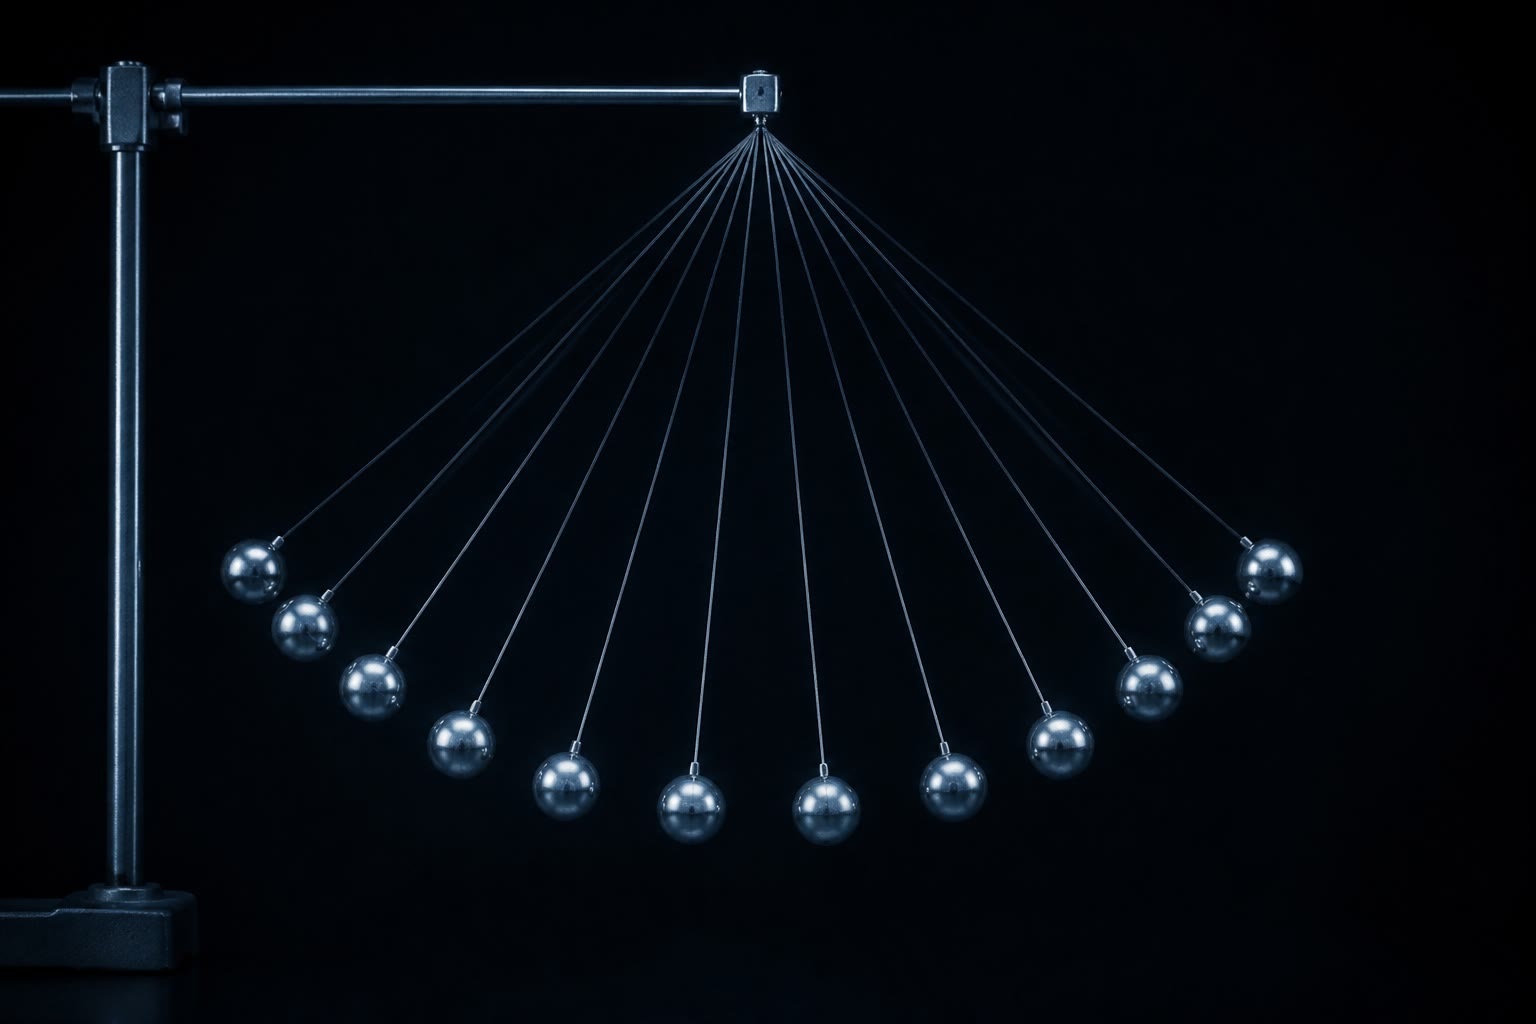
\includegraphics[width=0.58\linewidth]{images/book5/ai/b5-02-pendulum-strobe.jpg}

{\small स्ट्रोब-प्रकाश में देखा गया लोलक: स्थितियाँ पलट-बिंदुओं के पास भीड़ लगा देती हैं, जहाँ गोलक ठहरता है, और तल पर फैल जाती हैं, जहाँ वह जल्दी में रहता है --- यह उसी कला-समष्टि चित्र का छायाचित्र है जिसे यह अध्याय समीकरणों से खींचता है।}
\end{omfigure}

\section{अभ्यास}

\begin{exercise}[$\star$]\label{exo:b3:hamiltonian-mechanics:1}
स्प्रिंग पर द्रव्यमान के लिए: (क) $H$ को $L$ से बनाइए और जाँचिए कि $H =
E_k + E_p$; (ख) \omterm{def:b3:hamiltonian-mechanics:hamiltonian}{विहित समीकरण} लिखिए और जाँचिए कि वे
$\ddot x = -\omega^2x$ की पुनरुत्पत्ति करते हैं; (ग) दिखाइए कि
प्रक्षेप-पथ $(x, p)$ तल में दीर्घवृत्त हैं, और ऊर्जा $E$ पर उनके
अर्ध-अक्ष दीजिए; (घ) किस अर्थ में निरूपक बिंदु दक्षिणावर्त चलता है?
\end{exercise}

\begin{exercise}[$\star$]\label{exo:b3:hamiltonian-mechanics:2}
पिछले अध्याय के घूमते वलय पर मनके के लिए $L =
\tfrac12 mR^2\dot\theta^2 + \tfrac12 m\omega^2R^2\sin^2\theta +
mgR\cos\theta$ है। (क) $p$ और $H$ निकालिए। (ख) क्या $H$ संरक्षित है?
क्या वह यांत्रिक ऊर्जा है? (ग) $H$ के तलवक्र $\omega^2 < g/R$ और
$\omega^2 > g/R$ के लिए खींचिए, उसी अध्याय के प्रभावी विभव की सहायता से।
(घ) द्रुत स्थिति में केंद्र, काठी बिंदु और \omterm{def:b3:hamiltonian-mechanics:portrait}{पृथक्कारी वक्र}
पहचानिए।
\end{exercise}

\begin{exercise}[$\star$]\label{exo:b3:hamiltonian-mechanics:3}
कोई गेंद फर्श पर प्रत्यास्थ रूप से उछलती है, $H = p^2/2m + mgz$ ($z >
0$)। (क) एक उड़ान का और फिर पूरी उछल-कूद का कला-प्रक्षेप-पथ खींचिए।
(ख) प्रत्यास्थ उछाल निरूपक बिंदु के साथ क्या करता है? (ग) अधिकतम
ऊँचाई $z_{\max}$ के लिए घिरा क्षेत्रफल और \omterm{def:b3:lagrangian-mechanics:action}{क्रिया} $I$ निकालिए। (घ)
बोर--ज़ोमरफ़ेल्ट नियम $\oint p\,\dd z = nh$ किसी उछलते न्यूट्रॉन ($m =
\qty{1.67e-27}{kg}$) पर लगाने से क्वांटीकृत उछाल-ऊँचाइयाँ मिलती हैं:
सबसे नीची का आकलन कीजिए, और 2002 के गुरुत्वीय क्वांटम-अवस्था प्रयोग
में मापी गई \qty{15}{\micro m} से तुलना कीजिए।
\end{exercise}

\begin{exercise}[$\star$]\label{exo:b3:hamiltonian-mechanics:4}
केवल विहित संबंधों से निकालिए: (क) $\{x^2, p\}$; (ख)
$\{xp, H\}$, जहाँ $H = p^2/2m + E_p(x)$, और दोनों पदों की व्याख्या
कीजिए (यही कोष्ठक \emph{विरियल प्रमेय} चलाता है); (ग) $\{L_z, x\}$ और
$\{L_z, p_x\}$; (घ) दिखाइए कि यदि $\{f, H\} = 0$ और $\{g, H\} = 0$ हो
तो $\{f, g\}$ भी संरक्षित है (याकोबी सर्वसमिका का उपयोग कीजिए, जो
स्वीकृत है: $\{f,\{g,h\}\} + \{g,\{h,f\}\} + \{h,\{f,g\}\} = 0$)।
\end{exercise}

\begin{exercise}[$\star\star$]\label{exo:b3:hamiltonian-mechanics:5}
अपने \omterm{def:b3:hamiltonian-mechanics:portrait}{पृथक्कारी वक्र} के निकट लोलक। (क) \omterm{def:b3:hamiltonian-mechanics:portrait}{पृथक्कारी वक्र} की ऊर्जा और उस पर
अधिकतम $|p|$ दीजिए। (ख) दिखाइए कि \omterm{def:b3:hamiltonian-mechanics:portrait}{पृथक्कारी वक्र} पर $p =
\pm 2m\ell^2\omega_0\cos(\theta/2)$ है, जहाँ $\omega_0 = \sqrt{g/\ell}$।
(ग) $\dot\theta = p/m\ell^2$ का उपयोग करके दिखाइए कि $\theta$ से शीर्ष
तक का समय लघुगणकीय रूप से अपसरित होता है। (घ) \omterm{def:b3:hamiltonian-mechanics:portrait}{पृथक्कारी वक्र} से ज़रा
नीचे छोड़ा गया कोई वास्तविक लोलक उलटी स्थिति के पास एक लंबे क्षण तक
टिका रहता है और फिर लौटता है --- इसका संबंध (ग) से जोड़िए, और हर काठी
बिंदु के पास दिखने वाले मंदन से भी।
\end{exercise}

\begin{exercise}[$\star\star$]\label{exo:b3:hamiltonian-mechanics:6}
चुंबकीय क्षेत्र में किसी आवेशित कण का $H = (\vect p -
q\vect A)^2/2m$ है, जहाँ $\vect p$ पिछले अध्याय का विहित संवेग है।
(क) $\vect A = \tfrac12
B(-y, x, 0)$ के लिए \omterm{def:b3:hamiltonian-mechanics:hamiltonian}{विहित समीकरण} लिखिए और जाँचिए कि वे साइक्लोट्रॉन
गति देते हैं। (ख) दिखाइए कि $H =
\tfrac12 m\vect v^{\,2}$: चुंबकीय क्षेत्र कोई कार्य नहीं करता। (ग)
दोनों संरक्षित राशियों $\pi_x = p_x - \tfrac12
qBy$ और $\pi_y = p_y + \tfrac12 qBx$ का कोष्ठक निकालिए (पहले जाँचिए
कि प्रत्येक संरक्षित है), और दिखाइए कि $\{\pi_x, \pi_y\} = -qB$: दो
संरक्षित राशियाँ जिनका कोष्ठक एक अचर है। (घ)
\cref{exo:b3:hamiltonian-mechanics:4}(घ) का उपयोग करके समझाइए कि उनसे
किसी तीसरी स्वतंत्र संरक्षित राशि की अपेक्षा क्यों नहीं थी।
\end{exercise}

\begin{exercise}[$\star\star$]\label{exo:b3:hamiltonian-mechanics:7}
ल्यूविल, हाथ से। (क) स्वतंत्र कण के लिए प्रवाह $q \to q +
pt/m$, $p \to p$ है: दिखाइए कि कोई आयत उसी क्षेत्रफल का
समांतर चतुर्भुज बन जाता है। (ख) हरात्मक दोलक के लिए दिखाइए कि प्रवाह
एक घूर्णन है (उपयुक्त मात्रकों में) और निष्कर्ष निकालिए। (ग)
\emph{अवमंदित} दोलक $\ddot x = -\omega^2x - \gamma\dot x$ के लिए
$(x, v)$ तल में प्रवाह का अपसरण लिखिए और दिखाइए कि क्षेत्रफल
$\eu^{-\gamma t}$ की तरह सिकुड़ते हैं: अवमंदन
\omterm{def:b3:hamiltonian-mechanics:hamiltonian}{हैमिल्टोनियन} नहीं है। (घ) खोया हुआ क्षेत्रफल भौतिक रूप से कहाँ ``जाता'' है?
\end{exercise}

\begin{exercise}[$\star\star$]\label{exo:b3:hamiltonian-mechanics:8}
किसी केंद्रीय विभव में समतलीय गति, $H = (p_r^2 + p_\varphi^2/r^2)/2m
+ E_p(r)$। (क) चारों \omterm{def:b3:hamiltonian-mechanics:hamiltonian}{विहित समीकरण} लिखिए। (ख) दिखाइए कि $\{
p_\varphi, H\} = 0$ और संरक्षण नियम पहचानिए। (ग) इसे किसी प्रभावी विभव
वाले एकविमीय त्रिज्य \omterm{def:b3:hamiltonian-mechanics:hamiltonian}{हैमिल्टोनियन} तक घटाइए। (घ)
$E_p = -k/r$ के लिए दिए गए $p_\varphi$ पर वृत्ताकार कक्षा का स्थान
बताइए और उसकी ऊर्जा दीजिए --- जिसका क्वांटन
\cref{pb:b3:hamiltonian-mechanics:1} में होगा।
\end{exercise}

\begin{exercise}[$\star\star$]\label{exo:b3:hamiltonian-mechanics:9}
(क) विहित संबंधों से $\{L_x, L_y\} = L_z$ जाँचिए। (ख)
चक्रीय क्रमचय से शेष दोनों कोष्ठक निकालिए। (ग) दिखाइए कि
$\{L^2, L_z\} = 0$। (घ) कोई दृढ़ पिंड स्वतंत्र रूप से घूमता है:
$H =
L^2/2J$ (गोलीय सममित जड़त्व) लेकर दिखाइए कि तीनों $L_i$ संरक्षित हैं;
और असमान जड़त्व-आघूर्णों वाले पिंड के लिए क्या होगा (कोष्ठकों से
गुणात्मक उत्तर दीजिए)?
\end{exercise}

\begin{exercise}[$\star\star\star$]\label{exo:b3:hamiltonian-mechanics:10}
पुराने क्वांटम स्तर। (क) दिखाइए कि $\oint p\,\dd q = nh$ को
हरात्मक दोलक पर लगाने से $E_n = n\hbar\omega$ मिलता है, इसके लिए
\cref{prop:b3:hamiltonian-mechanics:sho-action} का उपयोग कीजिए। (ख)
उसे लंबाई $a$ के संदूक में बंद कण पर लगाइए और ठीक-ठीक $E_n =
n^2h^2/8ma^2$ पुनः प्राप्त कीजिए। (ग) किसी द्विपरमाणुक अणु को दृढ़ता
$k = \qty{1.9e3}{N/m}$ और समानीत द्रव्यमान $\qty{1.14e-26}
{kg}$ (कार्बन मोनोऑक्साइड) वाले दोलक के रूप में लेकर $\hbar\omega$ को
eV में और $n = 1 \to 0$ उत्सर्जन की तरंगदैर्घ्य निकालिए; वह किस
वर्णक्रमीय परिसर में पड़ती है? (घ) सच्चे स्तर $(n + \tfrac12)\hbar\omega$
हैं: क्या छूटा हुआ आधा \emph{उत्सर्जित} तरंगदैर्घ्यों को बदलता है? कौन-सा
प्रयोग शून्य-बिंदु वाले आधे को पकड़ता है?
\end{exercise}

\begin{exercise}[$\star\star\star$]\label{exo:b3:hamiltonian-mechanics:11}
$E/\omega$ की रुद्धोष्म निश्चरता, व्युत्पन्न। ऐसी स्प्रिंग पर द्रव्यमान
जिसकी दृढ़ता $k(t)$ धीरे-धीरे बढ़ती है। (क) दिखाइए कि यथार्थ गति के
अनुदिश $\dot E = \tfrac12\dot k\,
x^2$। (ख) नियत $k$ पर एक आवर्तकाल का औसत लीजिए:
$\langle\tfrac12 kx^2\rangle = E/2$ का उपयोग करके दिखाइए कि $\langle\dot E\rangle
= \dot k\,E/2k$। (ग) निष्कर्ष निकालिए कि $\dd\ln E = \tfrac12\dd\ln k = \dd\ln
\omega$, अतः $E/\omega$ अचर है। (घ) आयाम $\theta_0 = 5^\circ$ से
झूलते किसी लोलक की डोरी \qty{1.0}{m} से \qty{0.5}{m} तक धीरे-धीरे छोटी
की जाती है: नया आयाम और वह गुणक ज्ञात कीजिए जिससे उसकी ऊर्जा बढ़ी, और
बताइए कि ऊर्जा कहाँ से आई।
\end{exercise}

\begin{exercise}[$\star\star\star$]\label{exo:b3:hamiltonian-mechanics:12}
लोलक के \omterm{def:b3:hamiltonian-mechanics:portrait}{पृथक्कारी वक्र} के भीतर का क्षेत्रफल क्वांटम अवस्थाओं की एक
संख्या है। (क) दिखाइए कि \omterm{def:b3:hamiltonian-mechanics:portrait}{पृथक्कारी वक्र} के चारों ओर $\oint p\,\dd\theta$
$16m\ell^2\omega_0$ के बराबर है। (ख) बोर--ज़ोमरफ़ेल्ट नियम से
\omterm{def:b3:hamiltonian-mechanics:portrait}{पृथक्कारी वक्र} से नीची ऊर्जाओं वाली क्वांटम अवस्थाओं की संख्या $N \approx
16m\ell^2\omega_0/h$ है: \qty{10}{cm} की डोरी पर एक ग्राम के द्रव्यमान
के लिए उसका मान निकालिए। (ग) अमोनिया जैसे आणविक दोलक के लिए उसका मान
निकालिए: $m \sim \qty{1e-26}{kg}$, $\ell \sim \qty{1e-10}{m}$,
$\omega_0 \sim \qty{1e14}{rad/s}$। (घ) निष्कर्ष निकालिए: उस यांत्रिकी
की, जिसे $\hbar$ चाहिए, और उसकी जिसे नहीं चाहिए, सीमा कहाँ है?
\end{exercise}

\section{समस्या: पुरानी क्वांटम सिद्धांत और हाइड्रोजन परमाणु}

\begin{problem}[{सप्ताहांत समस्या --- कला समष्टि का क्वांटन, रिडबर्ग
का तौल}]\label{pb:b3:hamiltonian-mechanics:1}
1913 में बोर ने हाइड्रोजन का वर्णक्रम ग्रह-यांत्रिकी और एक क्वांटम
नियम से निकाला; ज़ोमरफ़ेल्ट ने पहचाना कि वह नियम कला-समष्टि के
क्षेत्रफल के विषय में एक कथन है। यह समस्या उनकी गणना को इस अध्याय के
औज़ारों से फिर से खड़ा करती है। आँकड़े: $m_{\text{e}} =
\qty{9.11e-31}{kg}$, $e = \qty{1.60e-19}{C}$, $1/4\pi\varepsilon_0 =
\qty{8.99e9}{N.m^2/C^2}$, $h = \qty{6.63e-34}{J.s}$, $c =
\qty{3.00e8}{m/s}$। $k = e^2/4\pi\varepsilon_0$ लिखिए।

\medskip\noindent\textbf{भाग I --- केप्लर \omterm{def:b3:hamiltonian-mechanics:hamiltonian}{हैमिल्टोनियन}।}
कोई इलेक्ट्रॉन किसी नियत प्रोटॉन के चारों ओर समतल में चलता है।
\begin{enumerate}
  \item प्रोटॉन को नियत मानने का औचित्य दीजिए (द्रव्यमान-अनुपात), और
        \omterm{def:b3:hamiltonian-mechanics:hamiltonian}{हैमिल्टोनियन} $H = \dfrac{p_r^2}{2m_{\text{e}}} +
        \dfrac{p_\varphi^2}{2m_{\text{e}}r^2} - \dfrac{k}{r}$ लिखिए।
  \item चारों \omterm{def:b3:hamiltonian-mechanics:hamiltonian}{विहित समीकरण} लिखिए।
  \item दिखाइए कि $p_\varphi$ संरक्षित है और उसे नाम दीजिए।
  \item त्रिज्य गति को प्रभावी विभव
        $U_{\text{प्र}}(r) = p_\varphi^2/2m_{\text{e}}r^2 - k/r$ तक
        घटाइए और उसका रेखाचित्र बनाइए।
  \item वृत्ताकार कक्षा का स्थान बताइए: $r_{\text{c}} =
        p_\varphi^2/m_{\text{e}}k$।
  \item दिखाइए कि उसकी ऊर्जा $E = -k/2r_{\text{c}} =
        -m_{\text{e}}k^2/2p_\varphi^2$ है, और जाँचिए कि वह स्थितिज
        ऊर्जा की आधी है (वर्ष 1 के खंड की गुरुत्वीय कक्षाओं वाला
        विरियल अनुपात)।
\end{enumerate}

\medskip\noindent\textbf{भाग II --- चिरसम्मत कक्षा।}
\begin{enumerate}[resume]
  \item त्रिज्या $r$ की वृत्ताकार कक्षा के लिए चाल $v$ और कक्षीय
        आवृत्ति $f_{\text{कक्ष}}$ को $r$ के फलनों के रूप में ज्ञात कीजिए।
  \item परमाणु के आकार की कक्षा, $r = \qty{0.05}{nm}$: $v$
        (और $v/c$), $f_{\text{कक्ष}}$, तथा ऊर्जा eV में निकालिए।
  \item उस कक्षा का कोणीय संवेग $p_\varphi$ निकालिए और उसकी तुलना
        $\hbar = h/2\pi$ से कीजिए: यह निकटता क्या सुझाती है?
  \item चिरसम्मत रूप से, परिक्रमा करता इलेक्ट्रॉन एक दोलायमान
        द्विध्रुव है और $f_{\text{कक्ष}}$ पर विकिरण करता है (वर्ष 2 का
        खंड); उसकी ऊर्जा लगभग \qty{1e-11}{s} में क्षीण हो जाती है।
        बताइए कि इससे परमाणुओं के विषय में कौन-सी दो घातक भविष्यवाणियाँ
        निकलती हैं, और इसके बदले क्या देखा जाता है।
  \item देखे गए वर्णक्रमों की कौन-सी विशेषता (विविक्त रेखाएँ, संयोजन
        नियम $1/\lambda = R_H(1/n^2 - 1/n'^2)$) ने विविक्त ऊर्जा-\emph{स्तरों}
        का सुझाव दिया?
  \item समझाइए कि ऐसी राशि के लिए, जो नियत सार्वत्रिक मान लेती हो,
        \emph{\omterm{prop:b3:hamiltonian-mechanics:adiabatic}{रुद्धोष्म निश्चर}} ही स्वाभाविक उम्मीदवार क्यों है
        (\cref{prop:b3:hamiltonian-mechanics:adiabatic} स्मरण कीजिए)।
\end{enumerate}

\medskip\noindent\textbf{भाग III --- क्वांटन।}
वृत्ताकार कक्षा की कोणीय गति पर ज़ोमरफ़ेल्ट का नियम लगाइए:
$\oint p_\varphi\,\dd\varphi = nh$, $n = 1, 2, 3, \dots$
\begin{enumerate}[resume]
  \item दिखाइए कि यह नियम $p_\varphi = n\hbar$ बन जाता है।
  \item अनुमत त्रिज्याएँ $r_n = n^2a_0$ निकालिए, जहाँ $a_0 =
        \hbar^2/m_{\text{e}}k$, और $a_0$ का मान निकालिए।
  \item अनुमत ऊर्जाएँ $E_n = -E_{\text{I}}/n^2$ निकालिए, जहाँ
        $E_{\text{I}} = m_{\text{e}}k^2/2\hbar^2$, और
        $E_{\text{I}}$ को जूल तथा eV में निकालिए।
  \item पहली कक्षा पर चाल निकालिए और जाँचिए कि $v_1/c =
        k/\hbar c \approx 1/137$ (सूक्ष्म-संरचना नियतांक)।
  \item कोई फ़ोटॉन किसी संक्रमण की ऊर्जा ले जाता है: रिडबर्ग सूत्र और
        $R_H = E_{\text{I}}/hc$ का मान निकालिए;
        मापे गए \qty{1.097e7}{m^{-1}} से तुलना कीजिए।
  \item संक्रमणों $2 \to 1$,
        $3 \to 2$ और $\infty \to 2$ की तरंगदैर्घ्य निकालिए; इनमें
        कौन-सी दृश्य है, और किस रंग की?
  \item आयनित हीलियम आयन He$^+$ नाभिकीय आवेश
        $2e$ वाला हाइड्रोजन है: $a_0$ और $E_{\text{I}}$ किस तरह
        मापित होते हैं, और उसकी $2 \to 1$ रेखा कहाँ पड़ती है?
\end{enumerate}

\medskip\noindent\textbf{भाग IV --- आमना-सामना।}
\begin{enumerate}[resume]
  \item कक्षीय आवृत्ति $f_{\text{कक्ष}}(n)$ और संक्रमण-आवृत्ति
        $\nu_{n \to n-1}$ को $n = 2$, $10$,
        $100$ के लिए निकालिए, और दिखाइए कि उनका अनुपात $1$ की ओर जाता
        है, ज्यों-ज्यों $n$ बढ़ता है।
  \item यही बोर का \emph{संगतता सिद्धांत} है: उसे एक वाक्य में
        बताइए।
  \item नियम $p_\varphi = n\hbar$ का आरंभ $n = 1$ से होता है: वृत्ताकार
        कक्षा के लिए $n = 0$ का क्या असंगत अर्थ होता?
  \item क्वांटम यांत्रिकी $E_n = -E_{\text{I}}/n^2$ को ठीक-ठीक रखेगी,
        फिर भी कक्षाओं को छोड़ देगी: दो ऐसे मापनीय तथ्य बताइए जिन्हें
        कक्षा-चित्र गलत बताता है (मूल अवस्था के कोणीय संवेग का मान;
        समान $n$ और भिन्न आकारों वाली अवस्थाओं का अस्तित्व)।
  \item म्युऑन $207$ गुना भारी इलेक्ट्रॉन है: म्युऑनी
        हाइड्रोजन के लिए $a_0^\mu$ और $E_{\text{I}}^\mu$ निकालिए, और
        समझाइए कि म्युऑनी परमाणु \emph{नाभिक} की जाँच क्यों करते हैं।
  \item नामित परिणाम का सार लिखिए: एक \omterm{prop:b3:hamiltonian-mechanics:adiabatic}{रुद्धोष्म निश्चर}, जिसे
        $h$ की पूर्ण संख्याओं के बराबर रखा जाए, $a_0 = \qty{52.9}{pm}$,
        $E_{\text{I}} = \qty{13.6}{eV}$ और हाइड्रोजन का वर्णक्रम चार
        अंकों तक दे देता है --- और सच्चे सिद्धांत को उसके दो केंद्रीय
        नियतांक सौंप देता है।
\end{enumerate}
\end{problem}
